\chapter{Slow data with timesynchronized and non timesynchronized sensor system}\label{sec:appendix_slow}

\begin{figure}[h]
  \begin{subfigure}[b]{0.42\textwidth}
    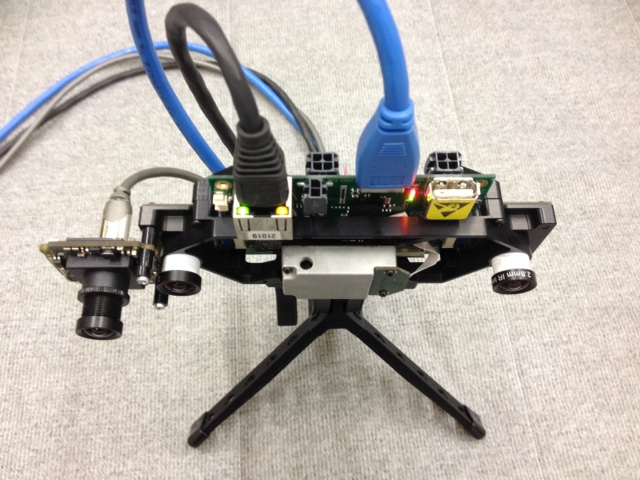
\includegraphics[width=\textwidth]{images/vi_bluefox.JPG}
    \caption{}
  \end{subfigure}
  \hfill
  \begin{subfigure}[b]{0.42\textwidth}
    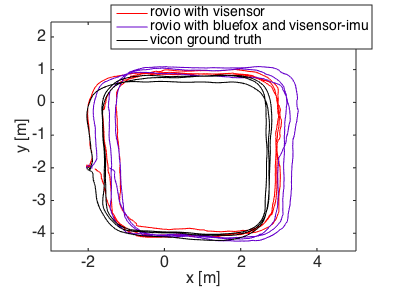
\includegraphics[width=\textwidth]{images/slow_2D.png}
    \caption{}
  \end{subfigure}
  \hfill
  \begin{subfigure}[b]{0.42\textwidth}
    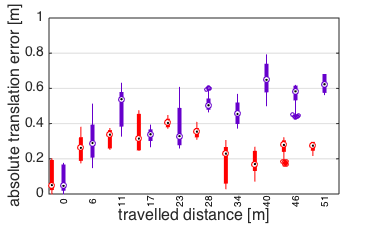
\includegraphics[width=\textwidth]{images/slow/slow_ate.png}
    \caption{}
  \end{subfigure}
  \begin{subfigure}[b]{0.42\textwidth}
    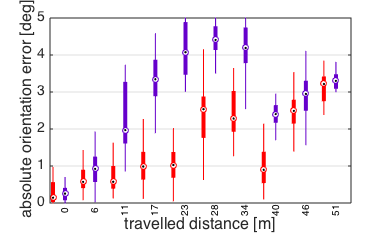
\includegraphics[width=\textwidth]{images/slow/slow_aoe.png}
    \caption{}
  \end{subfigure}
  \hfill
  \begin{subfigure}[b]{0.42\textwidth}
    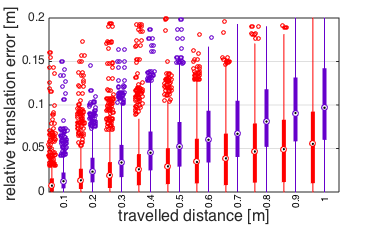
\includegraphics[width=\textwidth]{images/slow/slow_rte.png}
    \caption{}
  \end{subfigure}
  \hfill
  \begin{subfigure}[b]{0.42\textwidth}
    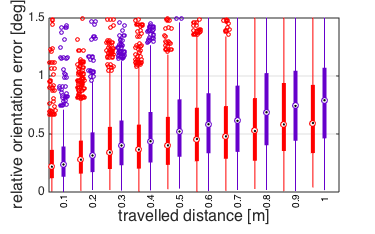
\includegraphics[width=\textwidth]{images/slow/slow_roe.png}
    \caption{}
  \end{subfigure}
   \caption{ROVIO results on the slow dataset with dynamics of $1.5\frac{m}{s}$ and $1\frac{rad}{s}$. ROVIO's tracking performance on the VI-sensor data (hardware-wise time synchronized) is better than on the data of the bluefox camera and the VI-sensor-IMU (hardware-wise non time synchronized). ROVIO is able to track for both the time synchronized and the non time synchronized data.}
   \label{pics:appendix_slow}
\end{figure}